\subsection{Spændingsforstærker}
\label{effekt_spaendingsforstaerker}
Spændingsforstærkerens opgave er at give en så stor spændingsforstærkning som muligt. Til dette projekts spændingsforstærker er der valgt en BC557B PNP-transistor koblet som en common-emitter. Koblingen af spændingsforstærkeren er vist på figur \ref{spaendingsforstaerker_diagram}

\begin{figure}[h]
\centering
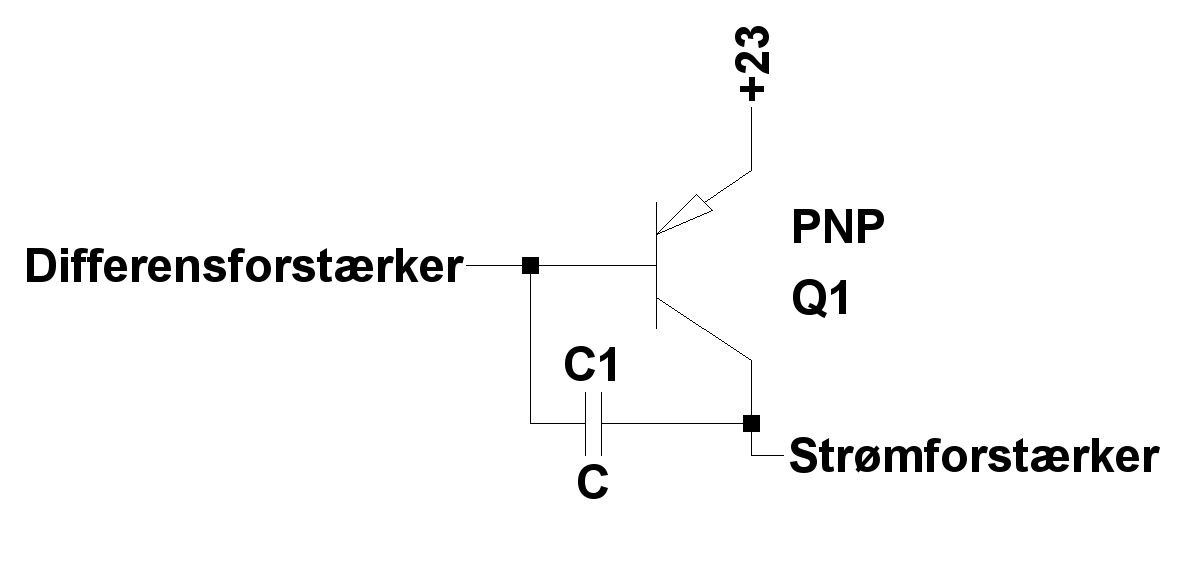
\includegraphics[scale=0.2]{teknisk/effektforstaerker/spaendingsforstaerker_diagram.png}
\caption{Diagram over opbygningen af spændingsforstærkeren.}
\label{spaendingsforstaerker_diagram}
\end{figure}

Forstærkningen i en commonemitter kobling er bestemt ved ligning (\ref{equ:spaendingsforstaerker1}) \cite{ael-mm7}%\fixme{Kilde: Jan analog elektronik mm7}

\begin{equation}
\label{equ:spaendingsforstaerker1}
A_v = -g_m \cdot R'_L
\end{equation}

For at beregne $g_m$ bruges ligning (\ref{equ:spaendingsforstaerker2}), hvor $I_c$ er den collectorstrøm som konstantstrømsgeneratoren trækker, og $V_T$ er sat til at være konstant $26~\mathrm{mV}$
\begin{equation}
\label{equ:spaendingsforstaerker2}
g_m = \frac{I_c}{V_T} = \frac{6~\mathrm{mA}}{26~\mathrm{mV}} = 230,8~\mathrm{mS}
\end{equation}

Nu skal $R'_L$ beregnes. $R'_L$ er defineret som den load spændingsforstærkeren ser. For at gøre det nemmere at beregne $R'_L$ er der lavet nogle antagelser. Første antagelse er at $V_\mathrm{be}$-multiplieren, når der kigges på AC, kan betragtes som en kortslutning. Næste antagelse er at konstantstrømsgeneratoren repræsentere en uendelig stor impedans, dette vil resultere i at den er meget større end de andre impedanser og derfor kan ses bort fra. Den sidste antagelse der er lavet er at kortslutningskredsløbet kan ses bort fra, idet dette kredsløb ikke er aktuelt, hvis systemet  kører som det skal. Med disse antagelser på plads kan impedansen $R'_L$ beregnes ud fra parallelkoblingen mellem de to darlingtontransistorer.

Det er derfor nødvendigt at finde den impedans som en darlingtontransistor  repræsenterer. Darlingtontransistorerne der er valgt til projektet er opbygget som vist på figur \ref{darlington_diagram}. I databladet for darlingtontransistorerne \cite{bdx33-34-datablad} er R1 angivet til typisk at være 10 k\ohm~og R2 til 150 \ohm.

\begin{figure}[h]
\centering
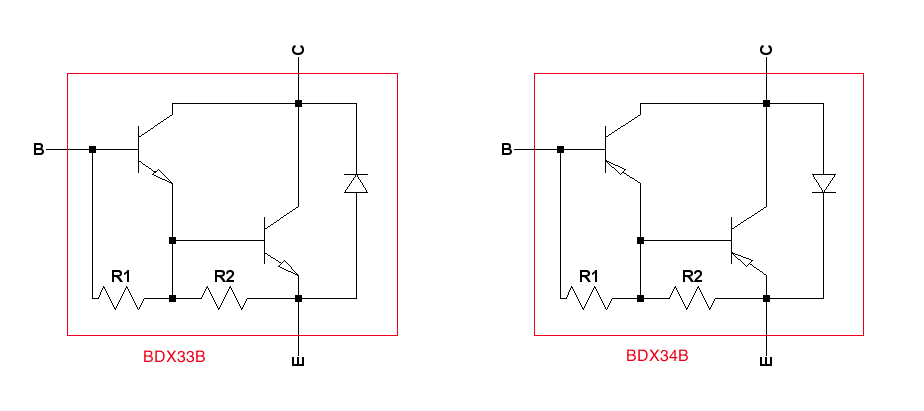
\includegraphics[scale = 0.4]{teknisk/effektforstaerker/darlingtontransistor_opbygning.png}
\caption{Diagram over opbygningen af darlingtontransistor BDX33B og BDX34B}
\label{darlington_diagram}
\end{figure}

For at gøre det nemmere at bestemme impedansen af darlingtontransistoren er det valgt at opfatte den som en enkelt supertransistor hvor $h_{\mathrm{fe}}= h_{\mathrm{fe}_1} \cdot h_{\mathrm{fe}_2}$ \cite{sedra-smith}. %\fixme{Kilde: sedra/smidth sixth edition side 525}
Der er også valgt at se bort fra de indre modstande i darlingtontransistoren. Når dette er valgt kan darlingtontransistoren i dette tilfælde opfattes som en transistor koblet som en commomcollector. Ud fra det kan der opstilles en simpel hybrid-$\pi$-model for supertransistoren som er vist i figur \ref{hybridpimodel_darlington}. Ud fra figur \ref{hybridpimodel_darlington} kan ligning (\ref{equ:spaendingsforstaerker3}) opsættes.

\begin{figure}[h]
\centering
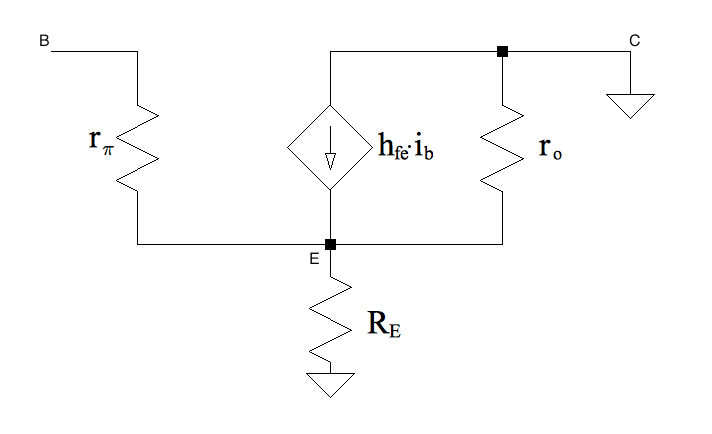
\includegraphics[scale=0.3]{teknisk/effektforstaerker/hybridpimodel.png}
\caption{Simpel småsignals hybrid-$\pi$-model  opstillet for supertransistor.}
\label{hybridpimodel_darlington}
\end{figure}
\begin{equation}
\label{equ:spaendingsforstaerker3}
v_b = i_b (r_{\pi} + (1+h_{\mathrm{fe}}) \cdot r_o||R_E) 
\end{equation}

Ligning (\ref{equ:spaendingsforstaerker3}) kan ved at dividere med $i_b$ på begge sider omskrives så det er indgangsimpedansen der regnes, dette er opstillet i ligning (\ref{equ:spaendingsforstaerker4})
\begin{equation}
\label{equ:spaendingsforstaerker4}
R_{\mathrm{in}} = r_{\pi} + (1+h_{\mathrm{fe}}) \cdot r_o||R_E 
\end{equation}

Fra databladet over darlingtontransistoren er $h_{\mathrm{fe}}$ angivet til minimum at være 750. Dette gør at  $(1+h_{\mathrm{fe}})$ kan erstattes med $h_{\mathrm{fe}}$ i formel (\ref{equ:spaendingsforstaerker4}), fordi $h_{\mathrm{fe}} >> 1$. Derudover er $r_o$ meget større end $R_e$ så denne kan også udelades af beregningen. $R_E$ er den impedans der sidder efter darlingtontransistoren, som i dette tilfælde er en serieforbindelse af $R_e$ + $R_L$, hvor $R_e$ er den termiske modstand og $R_L$ er den load højtaleren repræsentere. Med disse betragtninger kan ligning (\ref{equ:spaendingsforstaerker4}) forsimples til ligning (\ref{equ:spaendingsforstaerker5}).
\begin{equation}
\label{equ:spaendingsforstaerker5}
R_{\mathrm{in}} = r_{\pi} + h_{\mathrm{fe}} \cdot (R_e + R_L)
\end{equation}

Transistorparameteren $r_{\pi}$ er givet ved ligning (\ref{equ:spaendingsforstaerker6}).
\begin{equation}
\label{equ:spaendingsforstaerker6}
r_{\pi} = h_{\mathrm{fe}} \cdot \frac{1}{g_m}
\end{equation}

Ligning (\ref{equ:spaendingsforstaerker6} ) indsættes nu i ligning (\ref{equ:spaendingsforstaerker5}) og indgangsimpedansen for darlingtontransistoren beregnes.
\begin{equation}
\label{equ:spaendingsforstaerker7}
R_{\mathrm{in}} = \frac{h_{\mathrm{fe}}}{g_m} + h_{\mathrm{fe}} \cdot R_E = \frac{750}{230,8~\mathrm{mS}} + 750 \cdot (0,62~\ohm + 8~\ohm) = 9,76~\mathrm{k}\ohm  
\end{equation}

I ligning (\ref{equ:spaendingsforstaerker7}) får vi indgangsimpedansen for en darlingtontransistor til at være 9,76 k\ohm. Den load $R'_L$ som spændingsforstærkeren ser er den ene af de to darlingtontransistorer i parallel med konstantstrømsgeneratoren. Dette fremkommer fordi der ses bort fra hvileområdet, hvor begge darlingtontrasistorer er aktive og kun ses på situationen, hvor der er fuld udstyring på en af transistorerne. Derfor er den samledes impedans spændingsforstærkeren ser givet ved ligning (\ref{equ:spaendingsforstaerker8})
\begin{equation}
\label{equ:spaendingsforstaerker8}
R'_L = R_{\mathrm{in}}||R_{\mathrm{const}} = 9,76~\mathrm{k}\ohm||1,85~\mathrm{M}\ohm = 9,70~\mathrm{k}\ohm
\end{equation}  

Med $R'_L$ for spændingsforstærkeren fundet kan forstærkningen som før nævnt findes ved $A_v = -g_m \cdot R'_L$ og er udregnet i ligning (\ref{equ:spaendingsforstaerker9})
\begin{equation}
\label{equ:spaendingsforstaerker9}
A_v = -g_m \cdot R'_L = 230,8~\mathrm{mS} \cdot 9,70~\mathrm{k}\ohm = -2240,78
\end{equation}

Hermed er forstærkningen i spændingsforstærkeren beregnet til at være 2240,78 med et fasedrej på 180\degree .